\documentclass[a4paper, 12pt]{article}
\usepackage{graphicx}
\usepackage[slovene]{babel}
\usepackage[utf8]{inputenc}
\usepackage[T1]{fontenc}
\usepackage{lmodern}
\usepackage{amsmath, amssymb}
\usepackage{xcolor}
\usepackage[table]{xcolor}




\newtheorem{izrek}{Izrek}[section]

%\theoremstyle{definition}
\newtheorem{definicija}{Definicija}[section]

\newtheorem{opomba}{Opomba}[section]

\newtheorem{lema}{Lema}[section]

\newtheorem{trditev}{Trditev}[section]




\title{
    Distance vector of non tubical nanotube fullerenes of type-(5-0)
}

\author{Amanda Babič, Aljaž Flus \\
        {\small Mentorja Riste Škrekovski, Janoš Vidali}}
\date{\today}


\begin{document}

\maketitle

\newpage

\section{Uvod}

\begin{definicija}
    Vektor razdalje $d_{u}$ je vektor, katerega $i$-ta koordinata predstavlja število vozlišč, ki so od izbranega vozlišča $u$ oddaljeni natanko za $i$. 
\end{definicija}

\begin{definicija}
    Graf fulerena je 3-povezan, 3-regularen ravninski graf, sestavljen izključno iz petkotnih in šestkotnih ploskev.
\end{definicija}

\begin{opomba}
    Po Eulerjevi formuli je število petkotnih ploskev vedno 12.
\end{opomba}

\begin{definicija}
    Z $L_{0}$ začetni sloj kot množico vozličš, ki so sosednji s petkotnikom $p$, ki je središčni petkornik na začetku našega nanotuba 
    in definiramo s $F_0 = \{p\}$. Za vsak $j = 1, \dots , k$ množica plasti $F_j$ vsebuje vse plasti, ki so sosednje z vozlišči iz $L_{j-1}$ 
    in niso v $F_{j-1}$. Podobno $L_j$ vsebuje vsa vozlišča, ki so sosednja plasti is $F_j$ in niso v $L_{j-1}$. Zato je nanotub sestavljen Iz 
    $k+1$ plasti, kjer $L_0$ in $L_{k}$ vsebujeta $5$ vozličš, vsaka vmesna plast pa vsebuje $10$ vozlišč.
\end{definicija}

\begin{definicija}
    Naj bo $e = uv$ povezava v grafu $C_{10k}$, kjer je $u \in L_{j-1}$ in $v \in L_j$. Vozlišču u rečemo odhodno vozlišče za $L_{j-1}$, 
    vozlišču $v$ pa pravimo da je prihodno vozlišče za $L_j$. Tukaj lahko opazimo, da imamo v vsaki plasti $5$ odhodnih in $5$ prihodnid vozlišč,
    ki se zaporedoma izmenjujejo.
\end{definicija}

\begin{definicija}
    Naj bo $G$ neprazen končen povezan graf in $v$ vozlišče v grafu $G$. Distančna particija $\pi_{d}(v)$ 
    relativno na $v$ je skupina disjunktnih množic:
    \begin{itemize}
        \item $D_{0} = {v},$
        \item $D_{i} = {u : d(v,u) = i}, i= 1,2,3, \dots , ecc(v),$ \\
        kjer je $ecc(v)$ ekscentričnost vozlišča $v$, t.j. $ecc(v) = \max\limits_{u \in V(G)} d(v,u)$

    \end{itemize}
\end{definicija}

\begin{definicija}
    Naj bo $G$ neprazen končen povezan graf in $v$ vozlišče v $G$. Vektor distančne particije $DV(v) \in \mathbb{N}^{diam(G)}$ za vozlišče $v$
    definiramo kot
    $$
    DV(v) = (n_{0}(v), n_{1}(v), \dots , n_{diam(G)}(v)),
    $$
    kjer je $n_{i}(v) = |D_{i}|$ za $i=0,1, \dots , ecc(v)$, in $n_{i}(v) = 0$ za $ecc(v) < i \leq diam(G)$.
\end{definicija}

V naslednjem delu poročila bomo zaradi večje preglednosti izpustili ničelne komponente vektorja $DV(v)$. Pripomnemo lahko še 
da bo $n_{0}(v) = 1$ za vsak $v \in V(G)$

\section{Preverjanje izrekov}

\begin{lema}
    Če imamo 
    $$
    diam(C_{10k}) = \begin{cases}
                    2k+1, k=2;\\
                    2k, k \in \{3,4\};\\
                    2k-1, k \geq 5.

                    \end{cases}
    $$
    Potem lahko izračunamo ekscentričnosti. \\
    V kodi sva preverila to lemo za zečetnih 20 $k$ in so rezultati pravilni. Iz tega sklepamo da to velja za vse $k \in \mathbb{N}$
\end{lema}

\begin{lema}
    Za ekscentričnosti vozlišč v grafu $C_{10k}$ imamo:
    \begin{itemize}
        \item Če je $k=2$, potem je $ecc(v) = 5$ ta vse $v \in V(C_{10k})$.
        \item Če je $k=3$, potem je $ecc(v) = 6$ ta vse $v \in V(C_{10k})$.
        \item Če je $k \geq 4$ in $v \in L_{j}^{in} \cup L_{l-j}^{out}$ za $1 \leq j \leq \lfloor k/2 \rfloor$ potem je $$ecc(v) = 2(k-j) + \delta,$$
              kjer je $\delta = 2 $ za $(k,j) = (4,2)$, $\delta = 1$ za $(k , j) \in \{(4,1), (5,2), (6,3) \}$ in $\delta = 0$ sicer.
        \item Če je $k \geq 4$ in $v \in L_{j}^{out} \cup L_{k-j}^{in}$ za $0 \leq j \leq \lfloor k/2 \rfloor$ potem je $$ecc(v) = 2(k-j) - 1 +\delta$$
        kjer je $\delta = 2 $ za $(k,j) \in \{(4,1), (5,2)\}$, $\delta = 1$ za $(k , j) \in \{(4,0), (5,1), (6,2), (7,3) \}$ in $\delta = 0$ sicer.
    \end{itemize}
\end{lema}

\textcolor{red}{Lemo 2 sva preverila in ugotovila, da velja za $k=2$ in $k=3$. Vendar pa se pri večjih vrednostih $k$ izkaže, da lema ne drži, pri čemer ni očitne rešitve, kako bi jo ustrezno popravila.}

Za $k \geq 2$ in za vsak $j=0,1, \dots , k$ plast $L_j$ razdeli naš nanotub na dva disjuntna dela. Lev del sestavljajo plasti $L_i$ za $i = 0,1,\dots , j-1$, desni
 del pa je sestavljen iz plasti $L_i$ za $I = j+1, \dots, k$. Z $L(v)$ označimo levo stran particije, z $R(v)$ pa desno stran. Z $D(v)$ pa označimo distančni vektor znotraj plasti $L_j$.

\begin{trditev}
    Naj bo $k \geq 2$ in naj bo $v$ vozlišče iz grafa $C_{10k}$ tak da velja $v \in L_j, 0 \leq j \leq k$. Potem velja
    $$
    D(v) = \begin{cases}
            (1,2,2), \text{če } j \in \{0, k \}, \\
            (1,2,2,2,2,1), \text{sicer}, 
            \end{cases}
    $$
    in 
    $$
            DV(v) = L(v) + D(v) + R(v).
    $$

\end{trditev}

Če imamo $u \in L_j^{in}$ in $v \in L_{k-j}^{out}$ zaradi simetrije velja $R(u) = L(v)$. Velja tudi obratno, če imamo $u \in L_j^{out}$ in 
$v \in L_{k-j}^{in}$ prav tako velja $R(u) = L(v)$. Zaradi tega je dovlj izračunati samo $L(v)$. Izračuni so objavljeni v Tabela 1.

\begin{table}
\centering
$\begin{array}{ |c|c|c| }
    \hline
    L(v) & v \in L_j^{in} & v \in L_j^{out}  \\
    \hline
    j = 1 & [0, 1, 2, 2, 0, 0] & [0, 0, 2, 2, 1, 0] \\
    \hline
    j = 2, k = 2 & [0, 1, 4, 6, 3, 1] &  \\
    \hline
    j = 2, k \geq 3 & [0, 1, 2, 4, 4, 3, 1] & [0, 0, 2, 3, 5, 4, 1] \\
    \hline
    j = 3, k = 3 & [0, 1, 4, 6, 6, 6, 2] & \\
    \hline
    j = 3, k \geq 4 & [0, 1, 2, 4, 5, 7, 5, 1] & [0, 0, 2, 3, 5, 6, 7, 2] \\
    \hline
    j = 4, k = 4 & [0, 1, 4, 6, 6, 6, 6, 5, 1] & \\
    \hline
    j = 4, k \geq 5 & [0, 1, 2, 4, 5, 7, 7, 7, 2] & [0, 0, 2, 3, 5, 6, 7, 6, 6] \\
    \hline
    j = 5, k = 5 & [0, 1, 4, 6, 6, 6, 6, 5, 6, 5] & \\
    \hline
    j = 5, k \geq 6 & [0, 1, 2, 4, 5, 7, 7, 7, 6, 6] & [0, 0, 2, 3, 5, 6, 7, 6, 6, 5, 5]\\
    \hline
    6 \leq j \leq k-1, k \geq 7 & [0, 1, 2, 4, 5, 7, 7, 7, 6, 6, 5^{\#2(j-5)}] & [0, 0, 2, 3, 5, 6, 7, 6, 6, 5^{\#2(j-4)}]\\
    \hline
    j = k, k \geq 7 & [0, 1, 4, 6, 6, 6, 6, 5, 6, 5^{\#(2k - 9)}] & \\
    \hline
\end{array}$
\caption{Vektorji distančne particije, kjer gledamo samo vektorje ki so levo od našega vozlišča. Notacija $\#5^k$ nam predstavlja število petic zapored na koncu vektorja.}
\end{table}

V Tabela 1 opazimo, da se distančni vektorji razlikujejo za vozlišča znotraj iste orbite. To je posledica dejstva, da so vozlišča lahko bodisi vhodna bodisi izhodna. Vidimo, da je prvo število v vseh vektorjih vedno enako $0$, 
saj upoštevamo le vozlišča v orbitah na levi strani izbranega vozlišča. Pri izhodnih vozliščih opazimo, da je tudi drugi element enak $0$, kar pomeni, da sta potrebni vsaj dve potezi, da zapustimo svojo orbito. Poleg tega opazimo, 
da se distančni vektorji od $k=7$ naprej stabilizirajo.


\begin{izrek}
Naj bo $k \geq 10$. Dodatno naj bo $x = \text{'in'}$, če je $k$ sod in $x = \text{'out'}$, če je $k$ lih. Tako lahko izračunamo vektorje distančne 
particije za vsa vozlišča $C_{10k}$. Te vektorji so napisani v Tabela 2.
\end{izrek}

\begin{table}
\color{red}
$\begin{array}{|c|c|}
    \hline
    & \text{Vektor distanc DV(v)}\\
    \hline    
    j = 0  \text{ in } v \in L_j^{out} & [1, 3, 6, 6, 6, 6, 6, 5, 6, 5^{\#(2k - 9)}] \\
    \hline
    j = 1, k \text{ sod }  \text{ in } v \in L_j^{in}  & [1, 3, 6, 7, 7, 7, 7, 6, 6, 5^{\#(2k - 12)}]        \\
    \hline
    j = 1, k \text{ sod }  \text{ in } v \in L_j^{out}  &  [1, 3, 6, 8, 8, 8, 7, 7, 6, 6, 5^{\#(2k - 10)}]       \\
    \hline
    j = 1, k \text{ lih }  \text{ in } v \in L_j^{in}  & [1, 3, 6, 8, 8, 8, 7, 7, 6, 6, 5^{\#(2k - 14)}]        \\
    \hline
    j = 1, k \text{ lih }  \text{ in } v \in L_j^{out}  &  [1, 3, 6, 7, 7, 7, 7, 6, 6, 5^{\#(2k - 12)}]       \\
    \hline
    j = 2, k \text{ sod }  \text{ in } v \in L_j^{in}  &  [1, 3, 6, 9, 11, 10, 8, 6, 6, 5^{\#(2k - 12)}]       \\
    \hline
    j = 2, k \text{ sod }  \text{ in } v \in L_j^{out}  &  [1, 3, 6, 9, 12, 12, 8, 7, 6, 6, 5^{\#(2k - 14)}]       \\
    \hline
    j = 2, k \text{ lih }  \text{ in } v \in L_j^{in}  &  [1, 3, 6, 9, 11, 10, 8, 6, 6, 5^{\#(2k - 14)}]       \\
    \hline
    j = 2, k \text{ lih }  \text{ in } v \in L_j^{out}  &  [1, 3, 6, 9, 12, 12, 8, 7, 6, 6, 5^{\#(2k - 16)}]       \\
    \hline
    j = 3, k \text{ sod }  \text{ in } v \in L_j^{in}  &  [1, 3, 6, 9, 12, 14, 14, 9, 6, 6, 5^{\#(2k - 16)}]       \\
    \hline
    j = 3 , k \text{ sod } \text{ in } v \in L_j^{out}  & [1, 3, 6, 9, 12, 14, 12, 7, 6, 5^{\#(2k - 14)}]        \\
    \hline
    j = 3 , k \text{ lih }  \text{ in } v \in L_j^{in}  &  [1, 3, 6, 9, 12, 14, 14, 9, 6, 6, 5^{\#(2k - 18)}]       \\
    \hline
    j = 3 , k \text{ lih }  \text{ in } v \in L_j^{out}  & [1, 3, 6, 9, 12, 14, 12, 7, 6, 5^{\#(2k - 16)}]        \\
    \hline
    j = 4 , k \text{ sod }  \text{ in } v \in L_j^{in}  &  [1, 3, 6, 9, 12, 14, 14, 13, 8, 5^{\#(2k - 16)}]       \\
    \hline
    j = 4 , k \text{ sod }  \text{ in } v \in L_j^{out}  &  [1, 3, 6, 9, 12, 14, 14, 13, 12, 6, 5^{\#(2k - 18)}]       \\
    \hline
    j = 4 , k \text{ lih }  \text{ in } v \in L_j^{in}  &  [1, 3, 6, 9, 12, 14, 14, 13, 8, 5^{\#(2k - 18)}]       \\
    \hline
    j = 4 , k \text{ lih }  \text{ in } v \in L_j^{out}  &  [1, 3, 6, 9, 12, 14, 14, 13, 12, 6, 5^{\#(2k - 20)}]       \\
    \hline
    j = 5, k>12, \text{sod }  \text{in } v \in L_j^{in}  & [1, 3, 6, 9, 12, 14, 14, 13, 12, 11, 10, 5^{\#(2k - 21)}]  \\
    \hline
    j = 5, k>12, \text{sod }  \text{in } v \in L_j^{out}  & [1, 3, 6, 9, 12, 14, 14, 13, 12, 11, 5^{\#(2k - 19)}]  \\
    \hline
    j = 5, k>13, \text{lih }  \text{in } v \in L_j^{in} &  [1, 3, 6, 9, 12, 14, 14, 13, 12, 11, 10, 5^{\#(2k - 23)}] \\
    \hline
    j = 5, k>13, \text{lih }  \text{in } v \in L_j^{out} & [1, 3, 6, 9, 12, 14, 14, 13, 12, 11, 5^{\#(2k - 21)}] \\
    \hline
    j > 5, k>14, \text{sod }  \text{in } v \in L_j^{out}  & [1, 3, 6, 9, 12, 14, 14, 13, 12, 11, 10^{\#(2j - 10)}, 5^{\#(2k - 4j + 1)}]  \\
    \hline
    j > 5, k>14, \text{sod }  \text{in } v \in L_j^{in}  & [1, 3, 6, 9, 12, 14, 14, 13, 12, 11, 10^{\#(2j - 9)}, 5^{\#(2k - 4j - 1)}] \\
    \hline
    j > 5, k>15, \text{lih }  \text{in } v \in L_j^{out} & [1, 3, 6, 9, 12, 14, 14, 13, 12, 11, 10^{\#(2j - 9)}, 5^{\#(2k - 4j - 3)}] \\
    \hline
    j > 5, k>15, \text{lih }  \text{in } v \in L_j^{in} & [1, 3, 6, 9, 12, 14, 14, 13, 12, 11, 10^{\#(2j - 10)}, 5^{\#(2k - 4j - 1)}] \\
    \hline
    j = \lfloor k/2 \lfloor, k \text{ sod }  \text{ za vsak } v \in L_j  & [1, 3, 6, 9, 12, 14, 14, 13, 12, 11, 10^{\#(k - 10)}, 5]        \\
    \hline
    j = \lfloor k/2 \lfloor, k \text{ lih }  \text{ za vsak } v \in L_j  & [1, 3, 6, 9, 12, 14, 14, 13, 12, 11, 10^{\#(k - 11)}, 5]        \\
    \hline
\end{array}$
\caption{Vektorji distančne particije za graf $C_{10k}$, kjer je $k \geq 10$. Notaciji $\#5^k$ in $\#10^k$, nam povejo število petic oziroma desetic na koncu distančnega vektorja}
\end{table}

V Tabela 2 lahko opazimo, da distančni vektor ni odvisen zgolj od tega, ali je vozlišče $v$ vhodno ali izhodno, temveč tudi od tega ali je $k$ sodo ali liho število.

\section{Indeksi na podlagi distanc v $(5,0)$ nanotubu}

V tem oddelku bomo testirali različne indekse ki jih izračunamo na podlagi distanc v grafu $C_{10k}$

\begin{definicija}
    Indeks ekscentrične povezanosti za graf $G$ izračunamo tako
    $$
    \xi_{c}(G) = \sum_{v \in V(G)}deg_G(v)ecc_G(v),
    $$
    kjer z $deg_G(v)$ označimo stopnjo vozlišča $v$ v grafu $G$.
\end{definicija}

\begin{definicija}
    Indeks sosednje ekscentričnosti povezanosti za graf $G$ izračunamo tako
    $$
    \xi^{ad}(G) = \sum_{v \in V(G)}\frac{SG(v)}{ecc_G(v)},
    $$
    kjer z $SG(v)$ označimo seštevek stopenj vozlišč, ki so sosenja vozlišču v.
\end{definicija}

\begin{definicija}
    Prvi Zagrebški indeks povezanosti je definiran kot
    $$
    \xi_{1}(G) = \sum_{uv \in E(G)}(ecc_G(u) + ecc_G(v)),
    $$
    in drugi Zagrebški indeks povezanosti je definiran kot
    $$
    \xi_{2}(G) = \sum_{uv \in E(G)}(ecc_G(u)ecc_G(v)).
    $$
\end{definicija}

\begin{izrek}
    Naj bo $k \geq 8$. Potem velja:
    \begin{enumerate}
        \item $\xi_{c}(C_{10k}) = 45k^2 - 15k$,
        \item $90 \cdot \ln(2) \leq \xi^{ad}(C_{10k}) \leq 90 \cdot (\ln(2k - 1) - \ln(k - 1))$,
        \item $\xi_{1}(C)_{10k} = 45k^2 - 15k$
        \item $\xi_{2}(C_{10k}) = 35k^3 - \frac{45}{2}k^2 + \delta,$ kjer \textcolor{red}{$\delta = -5k + 10$, če je $k$ sodo in $\delta = 15 / 2 - 5 k$, če je $k$ liho.} 
    \end{enumerate}
\end{izrek}

Ta izrek sva preverila in res drži v vseh primerih. \textcolor{red}{Opazila pa sva tudi da druga točka velja za $k \geq 6$.}

\begin{definicija}
    Wienerjev indeks je definiran kot vsota distanc v grafu $G$
    $$
    W(G) = \sum_{\{u,v\}\in V(G)}dist(u,v).
    $$
    Hiper Wienerjev indeks je definiran kot
    $$
    WW(G) = \sum_{\{u,v\}\in V(G)} (dist(u,v) + dist^2(u,v)).
    $$
    Recipročni komplementarni Wienerjev indeks je definiran kot
    $$
    RCW(G) = \sum_{\{u,v\}\in V(G)} \frac{1}{diam(G) + 1 - dist_G(u,v)}.
    $$
\end{definicija}




\begin{izrek}
    Naj bo $k \geq 10$ in $t$ tak, da velja $10 \leq t \leq 2k - 1$. Tedaj velja:
    \begin{alignat*}{2}
        W_1(C_{10k}) &= 15k,  &\quad W_2(C_{10k}) &= 30k, \\
        W_3(C_{10k}) &= 45k - 30, &\quad W_4(C_{10k}) &= 60k - 80, \\
        W_5(C_{10k}) &= 70k - 135, &\quad W_6(C_{10k}) &= 70k - 180, \\
        W_7(C_{10k}) &= 65k - 220, &\quad W_8(C_{10k}) &= 60k - 230, \\
        W_9(C_{10k}) &= 55k - 250, &\quad W_t(C_{10k}) &= 50k - 25t.
    \end{alignat*}
\end{izrek}

Izrek drži.

\begin{izrek}
    Naj bo $k \geq 10$. Tedaj velja:
    \begin{align*}
        W(C_{10k}) &= \frac{100}{3} k^3 + \frac{1175}{3} k - 670, \\
        WW(C_{10k}) &= \frac{100}{3} k^4 + \frac{100}{3} k^3 - \frac{25}{3} k^2 + \frac{10175}{3} k - 7200, \\
        RCW(G) &= R_k + 50k - 250.
    \end{align*}
\end{izrek}

\textcolor{red}{
Pravilna formula za $R_k$ v trditvi 7 je:
\begin{equation*}
    R_k = \sum_{i=1}^{9} \frac{W_i(C_{10k})}{2k - i}.
\end{equation*}
}
\begin{izrek}
    Naj bo $\alpha \in \mathbb{R} \setminus \{0,1\}$. Označimo
    \begin{equation*}
        W_9^\alpha = \sum_{t=1}^{9} t \cdot W_t(C_{10k}).
    \end{equation*}
    Tedaj velja:
    \begin{equation*}
        W_9^\alpha + L < W^\alpha(C_{10k}) < W_9^\alpha + P,
    \end{equation*}
    kjer sta $L$ in $P$ spodnja in zgornja meja, določeni na sledeč način:


    \begin{equation*}
        L =
        \begin{cases} 
            \frac{50k}{\alpha + 1} \left( (2k)^{\alpha + 1} - 10^{\alpha + 1} \right) - 
            \frac{25}{\alpha + 2} \left( (2k-1)^{\alpha + 2} - 9^{\alpha + 2} \right) & \text{če } \alpha < 0, \alpha \neq -1, -2 \\
    
            \frac{50k}{\alpha + 1} \left( (2k-1)^{\alpha + 1} - 9^{\alpha + 1} \right) - 
            \frac{25}{\alpha + 2} \left( (2k-1)^{\alpha + 2} - 9^{\alpha + 2} \right) & \text{če } 0 < \alpha < 1 \\
    
            \frac{50k}{\alpha + 1} \left( (2k-1)^{\alpha + 1} - 9^{\alpha + 1} \right) - 
            \frac{25}{\alpha + 2} \left( (2k)^{\alpha + 2} - 10^{\alpha + 2} \right) & \text{če } \alpha > 1 \\
    
            50k \left( \ln(2k) - \ln(10) \right) & \text{če } \alpha = -1 \\
    
            -50k \left( (2k)^{-1} - 10^{-1} \right) - 25 \left( \ln(2k-1) - \ln(9) \right) & \text{če } \alpha = -2
        \end{cases}
    \end{equation*}
    

    \begin{equation*}
        P =
        \begin{cases} 
            \frac{50k}{\alpha + 1} \left( (2k-1)^{\alpha + 1} - 9^{\alpha + 1} \right) - 
            \frac{25}{\alpha + 2} \left( (2k)^{\alpha + 2} - 10^{\alpha + 2} \right) & \text{če } \alpha < 0, \alpha \neq -1, -2 \\
    
            \frac{50k}{\alpha + 1} \left( (2k)^{\alpha + 1} - 10^{\alpha + 1} \right) - 
            \frac{25}{\alpha + 2} \left( (2k)^{\alpha + 2} - 10^{\alpha + 2} \right) & \text{če } 0 < \alpha < 1 \\
    
            \frac{50k}{\alpha + 1} \left( (2k)^{\alpha + 1} - 10^{\alpha + 1} \right) - 
            \frac{25}{\alpha + 2} \left( (2k-1)^{\alpha + 2} - 9^{\alpha + 2} \right) & \text{če } \alpha > 1 \\
    
            50k \left( \ln(2k-1) - \ln(9) \right) - 50k + 250 & \text{če } \alpha = -1 \\
    
            -50k \left( (2k-1)^{-1} - 9^{-1} \right) - 25 \left( \ln(2k) - \ln(10) \right) & \text{če } \alpha = -2
        \end{cases}
    \end{equation*}
    


    
\end{izrek}


{\color{red} 
   Kljub večkratnim preverjanjem in različnim pristopom nikakor ne uspe priti do pravilnega rezultata, 
   kjer bi izrek veljal. 
   
   Zanimivo pa je, da izrek drži za vse $\alpha$, razen za $\alpha = -2$, če odstranimo $W_9$ iz ocen:
}
\[
L < W^\alpha(C_{10k}) < P.
\]
{\color{red}
   To kaže na morebitno napačno vključitev $W_9$ v meje ali potrebo po drugačnem načinu upoštevanja tega člena. \\  
   Opazimo tudi, da ne velja vedno $ \text{L} < \text{P} $ (npr. pri $\alpha = -1$).
}


Na zagovoru bodo predstavljeni tudi različni indeksi in njihove lastnosti.
S pomočjo grafov bo analiza še bolj nazorna, kar omogoča boljše razumevanje strukture in povezav v nanotubih.

\textcolor{red}{OD TUKAJ NAPREJ JE VSE NOVO.}

Pogledali si bomo sledeče indekse:
\begin{enumerate}
    \item \textbf{Recipročno komplementarni Wienerjev indeks}:
    \[
    RCW(G) = \sum_{{u,v} \in V(G)} \frac{1}{d + 1 - \operatorname{dist}_G(u,v)}
    \]




Spodaj je prikazan graf Reciprocal Complementary Wiener indeksa glede na velikost grafa:

\begin{figure}[h!]
    \centering
    
\includegraphics[width=0.8\textwidth]{rcw_index_plot.png}
    \caption{Vrednosti $\text{RCW}(G)$ za različne velikosti grafa $C_{10k}$.}
    \label{fig:rcw}
\end{figure}

Rast je (z razliko pri majhnih k) linearna in stabilna. Razdalje so pri majhnih k bolj skoncentrirane in graf preide iz kompaktne strukture v bolj raztegnjeno strukturo. 
    
    \item \textbf{Sum-Balaban indeks}:
    \[
    SJ(G) = \frac{m}{m - n + 2} \sum_{uv \in E(G)} \frac{1}{(w(u) + w(v))^{1/2}}
    \]

    \begin{figure}[h!]
        \centering
        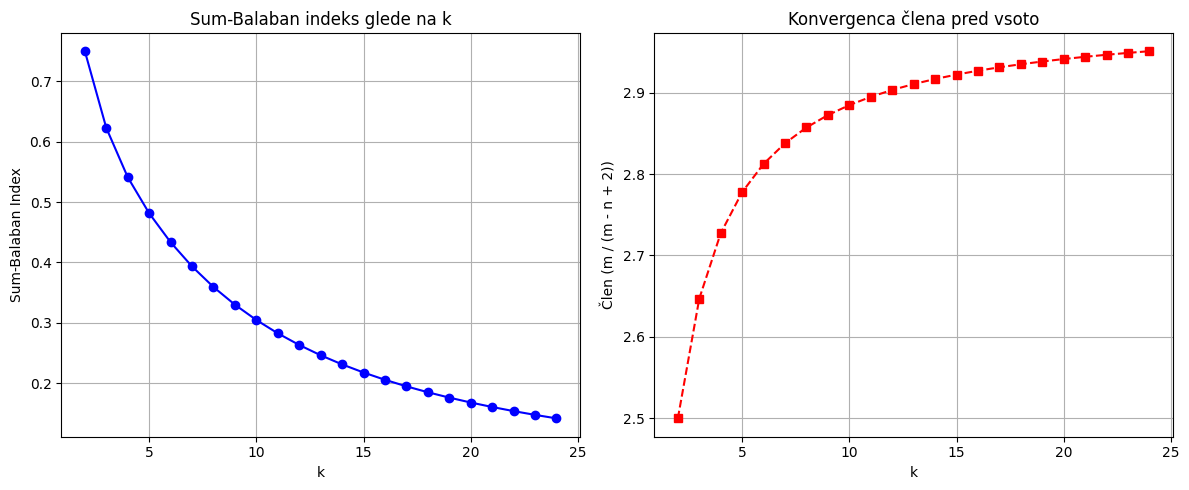
\includegraphics[width=0.8\textwidth]{sb_index_plot.png}
        \caption{Vrednosti RCW(G) za različne velikosti grafa C\{10k\}.}
        \label{fig:rcw}
    \end{figure}

    Opazimo, da člen pred vsoto konvergira k 3 (stabilno razmerje povezav in vozlišč). Indeks nam pove, kako so vozlišča povezana znotraj grafa. Nižja vrednost implicira kompakten graf in enakomerno, simetrično strukturo.
    
    \item \textbf{Generaliziran Wienerjev indeks}:
    \[
    W_{\lambda}(G) = \sum_{{u,v} \in V(G)} \operatorname{dist}^{\lambda}(u,v)
    \]
    

    \begin{figure}[h!]
        \centering
        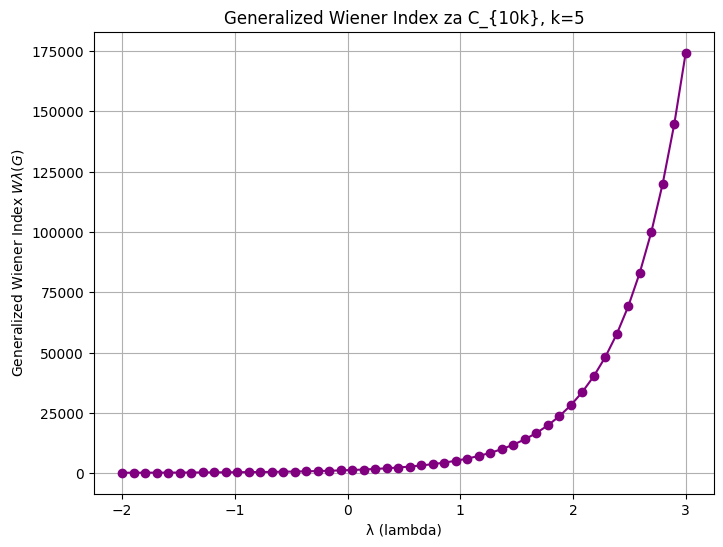
\includegraphics[width=0.8\textwidth]{gw_index_plot.png}
        \caption{Vrednosti RCW(G) za različne velikosti grafa C\{10k\}.}
        \label{fig:rcw}
    \end{figure}

    Opazimo da ne glede na lambdo indeks monotono raste, kar je smiselno, saj se število vozlišč povečuje. \
Pri lambdah blizu 1 je rast ekstremno hitra (skoraj eksponentna), pri negativnih je rast bistveno počasnejša, a še vedno monotono narašča.


    \item \textbf{Indeks ekscentrične povezanosti}:
    \[
    \xi_c(G) = \sum_{v \in V(G)} \deg_G(v) \cdot \operatorname{ecc}_G(v)
    \]
    \begin{figure}[h!]
        \centering
        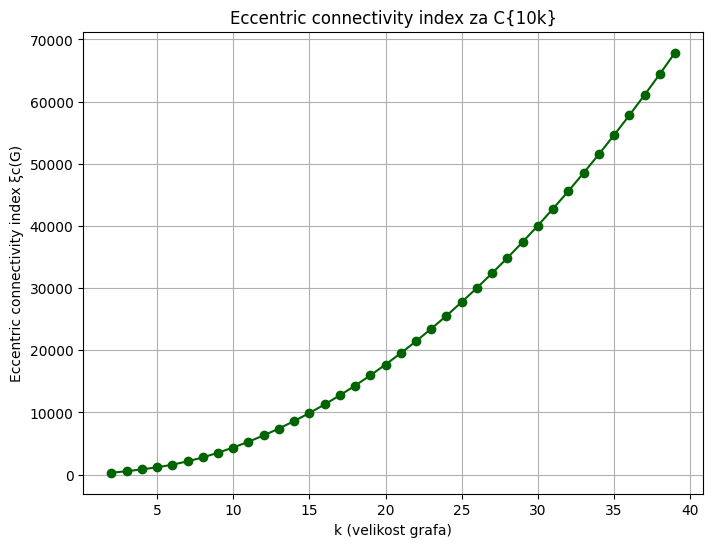
\includegraphics[width=0.8\textwidth]{ec_index_plot.png}
        \caption{Vrednosti RCW(G) za različne velikosti grafa C\{10k\}.}
        \label{fig:rcw}
    \end{figure}

    Ta indeks je odvisen od stopnje vozlišč in od ekscentričnosti vozlišč. Naš graf je 3-regularen, zato je v našem primeru indeks odvisen zgolj od ekscentričnosti. Tako rast indeksa odraža rast ekscentričnosti. Graf nam jasno kaže, da se z večanjem vozlišč graf razteguje v dolžino.

    \item \textbf{Indeks sosednje ekscentričnosti}:
    \[
    \xi_{\text{ad}}(G) = \sum_{v \in V(G)} \frac{\operatorname{SG}(v)}{\operatorname{ecc}_G(v)}
    \]
    

    \begin{figure}[h!]
        \centering
        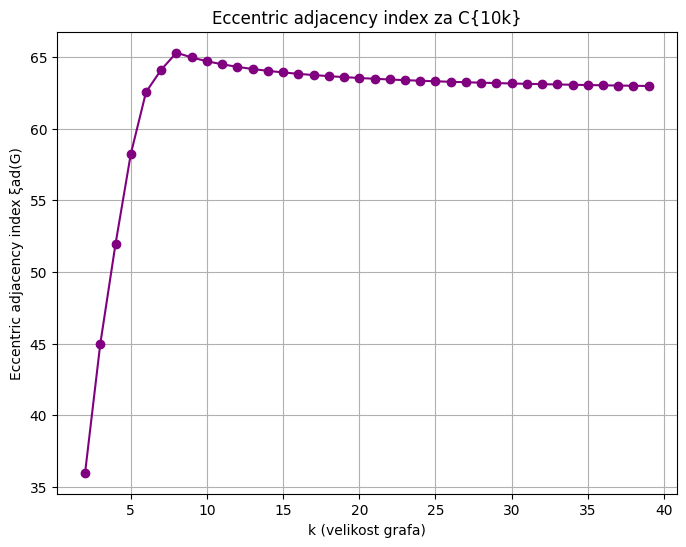
\includegraphics[width=0.8\textwidth]{ea_index_plot.png}
        \caption{Vrednosti RCW(G) za različne velikosti grafa C\{10k\}.}
        \label{fig:rcw}
    \end{figure}


    Ta indeks je odvisen od ekstentričnosti posameznega vozlišča in vsote stopenj njegovih sosedov. 
    Ko je k majhen, indeks hitro narašča. Ko dodamo samo nekaj orbital, se poveča vsota stopenj sosedov, ampak hkrati ekscentričnost še ni močno narasla, kar poveča indeks.
    Graf hitro doseže maksimum in nato se približuje določeni vrednosti. Ko k narašča, začnejo tudi ekscentričnosti vozlišč hitro naraščati, kar zmanjšuje indeks. zaradi regularnosti našega grafa pa se ta dva učinka medsebojno izravnata.

    Opazimo, da (po doseženem maksimumu) konvergira proti 62.


    \item \textbf{Prvi ekscentrični povezovalni indeks}:
    \[
    \xi_1(G) = \sum_{uv \in E(G)} (\operatorname{e}_G(u) + \operatorname{e}_G(v))
    \]

    \begin{figure}[h!]
        \centering
        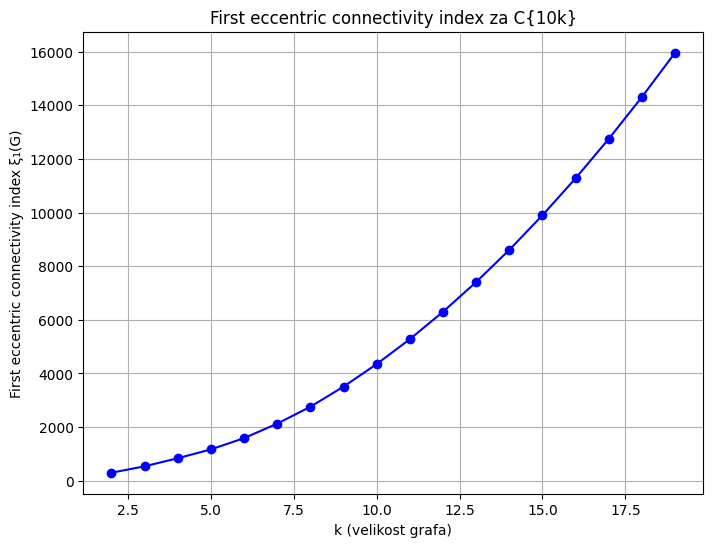
\includegraphics[width=0.8\textwidth]{fec_index_plot.png}
        \caption{Vrednosti RCW(G) za različne velikosti grafa C\{10k\}.}
        \label{fig:rcw}
    \end{figure}
    

    Indeks je odvisen od ekscentričnosti in števila povezav in narašča približno kvadratno. 
    \item \textbf{Drugi ekscentrični povezovalni indeks}:
    \[
    \xi_2(G) = \sum_{uv \in E(G)} (\operatorname{e}_G(u) \cdot \operatorname{e}_G(v))
    \]


    \begin{figure}[h!]
        \centering
        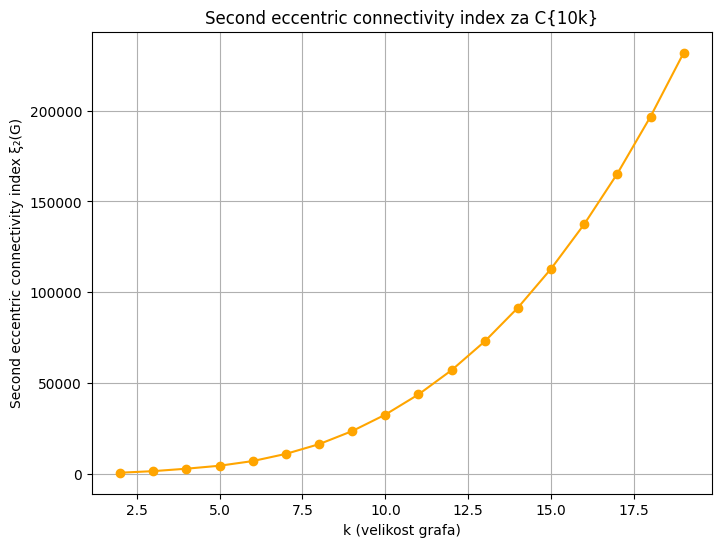
\includegraphics[width=0.8\textwidth]{sec_index_plot.png}
        \caption{Vrednosti RCW(G) za različne velikosti grafa C\{10k\}.}
        \label{fig:rcw}
    \end{figure}



    Indeks je odvisen od ekscentričnosti in števila povezav, enako kot pri prejšnjem primeru. Indeks uporablja produkt eksentričnosti, zato je pričakovana hitrejša rast kot prej, kar tudi graf potrjuje.
\end{enumerate}





 
\end{document}